\documentclass[journal,12pt,twocolumn]{IEEEtran}

\usepackage{setspace}
\usepackage{gensymb}
\singlespacing
\usepackage[cmex10]{amsmath}

\usepackage{amsthm}

\usepackage{mathrsfs}
\usepackage{txfonts}
\usepackage{stfloats}
\usepackage{bm}
\usepackage{cite}
\usepackage{cases}
\usepackage{subfig}

\usepackage{longtable}
\usepackage{multirow}

\usepackage{enumitem}
\usepackage{mathtools}
\usepackage{steinmetz}
\usepackage{tikz}
\usepackage{circuitikz}
\usepackage{verbatim}
\usepackage{tfrupee}
\usepackage[breaklinks=true]{hyperref}
\usepackage{graphicx}
\usepackage{tkz-euclide}

\usetikzlibrary{calc,math}
\usepackage{listings}
    \usepackage{color}                                            %%
    \usepackage{array}                                            %%
    \usepackage{longtable}                                        %%
    \usepackage{calc}                                             %%
    \usepackage{multirow}                                         %%
    \usepackage{hhline}                                           %%
    \usepackage{ifthen}                                           %%
    \usepackage{lscape}     
\usepackage{multicol}
\usepackage{chngcntr}

\DeclareMathOperator*{\Res}{Res}

\renewcommand\thesection{\arabic{section}}
\renewcommand\thesubsection{\thesection.\arabic{subsection}}
\renewcommand\thesubsubsection{\thesubsection.\arabic{subsubsection}}

\renewcommand\thesectiondis{\arabic{section}}
\renewcommand\thesubsectiondis{\thesectiondis.\arabic{subsection}}
\renewcommand\thesubsubsectiondis{\thesubsectiondis.\arabic{subsubsection}}


\hyphenation{op-tical net-works semi-conduc-tor}
\def\inputGnumericTable{}                                 %%

\lstset{
%language=C,
frame=single, 
breaklines=true,
columns=fullflexible
}
\begin{document}

\newcommand{\BEQA}{\begin{eqnarray}}
\newcommand{\EEQA}{\end{eqnarray}}
\newcommand{\define}{\stackrel{\triangle}{=}}
\bibliographystyle{IEEEtran}
\raggedbottom
\setlength{\parindent}{0pt}
\providecommand{\mbf}{\mathbf}
\providecommand{\pr}[1]{\ensuremath{\Pr\left(#1\right)}}
\providecommand{\qfunc}[1]{\ensuremath{Q\left(#1\right)}}
\providecommand{\sbrak}[1]{\ensuremath{{}\left[#1\right]}}
\providecommand{\lsbrak}[1]{\ensuremath{{}\left[#1\right.}}
\providecommand{\rsbrak}[1]{\ensuremath{{}\left.#1\right]}}
\providecommand{\brak}[1]{\ensuremath{\left(#1\right)}}
\providecommand{\lbrak}[1]{\ensuremath{\left(#1\right.}}
\providecommand{\rbrak}[1]{\ensuremath{\left.#1\right)}}
\providecommand{\cbrak}[1]{\ensuremath{\left\{#1\right\}}}
\providecommand{\lcbrak}[1]{\ensuremath{\left\{#1\right.}}
\providecommand{\rcbrak}[1]{\ensuremath{\left.#1\right\}}}
\theoremstyle{remark}
\newtheorem{rem}{Remark}
\newcommand{\sgn}{\mathop{\mathrm{sgn}}}
\providecommand{\abs}[1]{\vert#1\vert}
\providecommand{\res}[1]{\Res\displaylimits_{#1}} 
\providecommand{\norm}[1]{\lVert#1\rVert}
%\providecommand{\norm}[1]{\lVert#1\rVert}
\providecommand{\mtx}[1]{\mathbf{#1}}
\providecommand{\mean}[1]{E[ #1 ]}
\providecommand{\fourier}{\overset{\mathcal{F}}{ \rightleftharpoons}}
%\providecommand{\hilbert}{\overset{\mathcal{H}}{ \rightleftharpoons}}
\providecommand{\system}{\overset{\mathcal{H}}{ \longleftrightarrow}}
	%\newcommand{\solution}[2]{\textbf{Solution:}{#1}}
\newcommand{\solution}{\noindent \textbf{Solution: }}
\newcommand{\cosec}{\,\text{cosec}\,}
\providecommand{\dec}[2]{\ensuremath{\overset{#1}{\underset{#2}{\gtrless}}}}
\newcommand{\myvec}[1]{\ensuremath{\begin{pmatrix}#1\end{pmatrix}}}
\newcommand{\mydet}[1]{\ensuremath{\begin{vmatrix}#1\end{vmatrix}}}
\numberwithin{equation}{subsection}
\makeatletter
\@addtoreset{figure}{problem}
\makeatother
\let\StandardTheFigure\thefigure
\let\vec\mathbf
\renewcommand{\thefigure}{\theproblem}
\def\putbox#1#2#3{\makebox[0in][l]{\makebox[#1][l]{}\raisebox{\baselineskip}[0in][0in]{\raisebox{#2}[0in][0in]{#3}}}}
     \def\rightbox#1{\makebox[0in][r]{#1}}
     \def\centbox#1{\makebox[0in]{#1}}
     \def\topbox#1{\raisebox{-\baselineskip}[0in][0in]{#1}}
     \def\midbox#1{\raisebox{-0.5\baselineskip}[0in][0in]{#1}}
\vspace{3cm}
\title{Assignment 5}
\author{Vijay Varma - AI20BTECH11012}
\maketitle
\newpage
\bigskip
\renewcommand{\thefigure}{\theenumi}
\renewcommand{\thetable}{\theenumi}
%
Download latex-tikz codes from 
%
\begin{lstlisting}
https://github.com/KBVijayVarma/EE3900/tree/main/Assignment_5
\end{lstlisting}
%
Download python codes from 
%
\begin{lstlisting}
https://github.com/KBVijayVarma/EE3900/tree/main/Assignment_5/code
\end{lstlisting}
\section*{\textbf{Problem (Quadratic Forms Q.2.9)}}
Find the smaller area enclosed by the circle $\vec{x}^\top\vec{x}=4$ and the line $\myvec{1 & 1}\vec{x}=2$.
\section*{\textbf{Solution}}
General equation of circle is
\begin{align}
    \vec{x}^\top\vec{x}+2\vec{u}^\top\vec{x}+f=0 \\
    \norm{\vec{x}}^2+2\vec{u}_1^\top\vec{x}+f_1=0 \\
    \vec{x}^\top\vec{x} - 4 = 0 \\
    \vec{u}_1=\myvec{0\\0} \\
    f_1 = -4 \\
    \vec{O}_1 = \myvec{0\\0} \\
    r = \sqrt{\vec{u}_1^\top\vec{u}_1 - f_1} = \sqrt{4} \\
    \Rightarrow r = 2 \label{eq-8}
\end{align}
From \eqref{eq-8}, the points at which circle touches X-axis is $\myvec{-2\\0}$ and $\myvec{2\\0}$.

The direction vector of the given line $\myvec{1 & 1}\vec{x}=2$ is $\myvec{-1\\1}$.

\begin{figure}[!h]
\centering
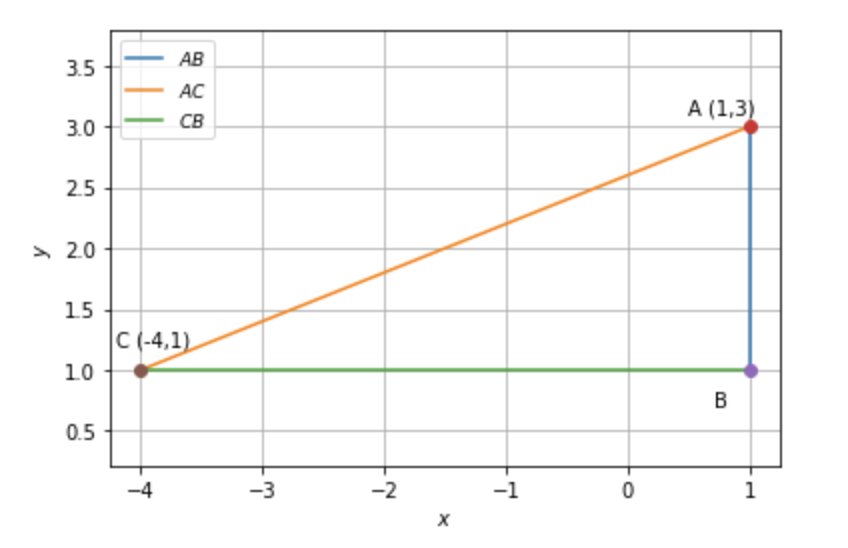
\includegraphics[width=\columnwidth]{fig.png}
\caption{Smaller area enclosed by line and circle}
\end{figure}

To find point $\vec{A}$ and $\vec{B}$, the parametric form of line is,
\begin{align}
    \vec{A}&=\vec{q}+\lambda\vec{m} \\
    &= \myvec{1\\1}+\lambda\myvec{-1\\1} \\
    \lambda^2 &= \frac{-f_1-\norm{\vec{q}}^2}{\norm{\vec{m}}^2} \\
    &= \frac{4-2}{2} = 1 \\
    \Rightarrow \lambda &= \pm 1
\end{align}
\begin{align}
    \vec{A} = \myvec{0\\2} \vec{B} = \myvec{-2\\0} \\
    \vec{O_1} = \myvec{0\\0} \\
    (\vec{A} - \vec{O_1}) = \myvec{0\\2} \\
    (\vec{B} - \vec{O_1}) = \myvec{-2\\0}
\end{align}
Inner product of $(\vec{A} - \vec{O_1})$ and $(\vec{A} - \vec{O_1})$ is given as: \\

\begin{align}
    (\vec{A} - \vec{O_1})^\top(\vec{B} - \vec{O_1}) = 0
\end{align}

Therefore, $(\vec{A} - \vec{O_1}) \perp (\vec{B} - \vec{O_1})$ \\

Smaller area enclosed by circle and line $\vec{AB}$ is: 

Area = (Area of circle in 2nd Quadrant) - (Area of right triangle formed by line AB, X and Y axis)

\begin{align}
    Area &= \frac{\pi\theta_1}{360}r^2 - \frac{1}{2}\times2\times2 \\
    &= \frac{90}{360}\times2^2 - 2 \\
    &= \pi - 2
\end{align}
Hence, the smaller area enclosed by the circle 

$\vec{x}^\top\vec{x}=4$ and the line $\myvec{1 & 1}\vec{x}=2$ is $(\pi - 2)$ square units.
\end{document}